\section{Progettazione Concettuale}
	
	\subsection{Strategia di Progetto}
		\emph{Top-down} per la realizzazione dello schema ad un adeguato livello di raffinamento. \emph{Inside-out} per la successiva correzione dello stesso.
		
		\emph{Questa sezione va ampliata e corretta}
		
	\subsection{Individuazione delle Entità Fondamentali}
		
		Dalle specifiche che abbiamo formulato risulta che uno dei punti fondamentali da affrontare è quello della memorizzazione dei preventivi emessi dall'attività.
		Ad ogni \emph{Prestazione} effettuata, corrisponde un \emph{Preventivo} precedentemente emesso.
		
		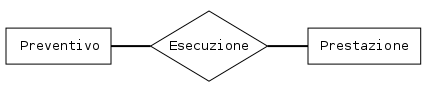
\includegraphics[width=11.5cm]{images/diagrams/preventivo_prestazione.png}
		
		Alla formulazione di ogni preventivo, si fa una stima dei componenti che si reputa saranno necessari per eseguire la prestazione preventivata. Non sempre tale previsione è completamente completamente esatta, generalmente i componenti effettivamente utilizzati in una prestazione sono diversi da quelli previsti in un preventivo.
		L'associazione tra i \emph{Componenti} e il \emph{Preventivo} risulta immediata.
		
		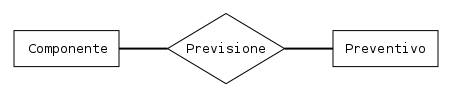
\includegraphics[width=11.5cm]{images/diagrams/preventivo_componente.png}
		
		Prima di esplicitare l'associazione tra le prestazioni eseguite ed i componenti effettivamente utilizzati, affrontiamo la questione degli ordini e del magazzino.
		
		L'acquisto di articoli presso un fornitore è formalizzato in un ordine, il quale, come da specifiche, è organizzato in più forniture, ovvero insiemi di articoli di uno stesso componente.
		Ad un \emph{Ordine} sono associate una o più \emph{Forniture} di articoli, ognuna delle quali fanno riferimento ad un \emph{Componente}.
		
		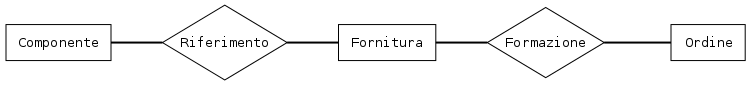
\includegraphics[width=11.5cm]{images/diagrams/componente_ordine.png}
		
		Il magazzino, nella realtà, è composto dai vari articoli acquistati che sono in attesa di essere utilizzati. La classificazione degli articoli avviene, in primo luogo per componente, in secondo luogo per fornitura d'appartenenza. Non vi è così il bisogno di registrare ogni articolo individualmente, ma basterà riferirsi alle relative forniture.
		Il \emph{Magazzino} è una composizione di \emph{Forniture} i cui articoli sono depositati in attesa di essere utilizzati.
		
		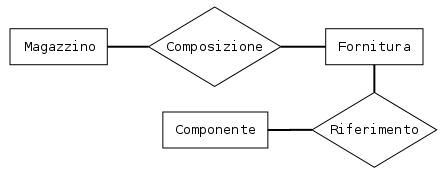
\includegraphics[width=11.5cm]{images/diagrams/magazzino_fornitura.png}
		
		Per identificare con precisione quali articoli sono stati utilizzati per l'esecuzione di una prestazione, sarà sufficiente riferirsi alla fornitura relativa agli stessi. Da questa si ottengono le informazioni sul componente (quindi il prezzo di vendita e il tempo di validità) e sulla data d'acquisto.
		Ad ogni utilizzo, si provvederà ad aggiornare le quantità rimanenti degli articoli delle forniture utilizzate.
		Per l'esecuzione di una \emph{Prestazione} si possono utilizzare gli articoli di più \emph{Forniture}.
		
		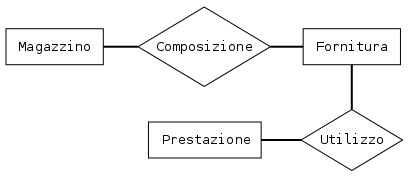
\includegraphics[width=11.5cm]{images/diagrams/prestazione_fornitura.png}
		
		Passiamo alla questione degli operatori. Una prestazione viene eseguita da uno o più operatori. Di ogni operatore si vuole tener traccia dei turni di lavoro effettuati.
		Alla \emph{Prestazione}, saranno associati uno o più \emph{Operatori} ad ognuno dei quali sono associati i relativi \emph{Turni} di lavoro.
		
		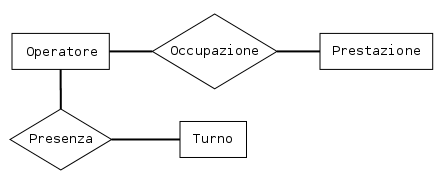
\includegraphics[width=11.5cm]{images/diagrams/operatore_turno_prestazione.png}
		
		Occupiamoci ora delle zone periferiche dello schema. Un preventivo viene effettuato quando un cliente richiede un intervento alla propria auto.
		Ad ogni \emph{Cliente} vengono associate una o più \emph{Autovetture}. Ogni \emph{Preventivo} si riferisce ad una specifica \emph{Autovettura}.
		
		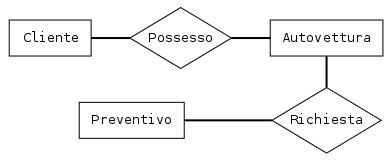
\includegraphics[width=11.5cm]{images/diagrams/cliente_autovettura_preventivo.png}
		
		Ogni \emph{Ordine} viene effettuato presso un \emph{Fornitore}.
		
		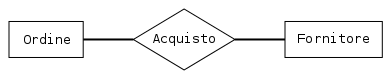
\includegraphics[width=11.5cm]{images/diagrams/ordine_fornitore.png}
		
		Notiamo che \emph{Cliente} rappresenta sia \emph{Privati} che \emph{Aziende} (rispettivamente, clienti non dotati di partita iva e clienti dotati di partita iva).
		
		\begin{center}
			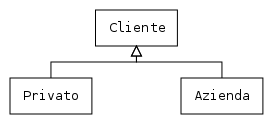
\includegraphics[width=9cm]{images/diagrams/cliente.png}
		\end{center}
		
		Inoltre \emph{Clienti}, \emph{Fornitori} ed \emph{Operatori} possono essere generalizzati dall'entità \emph{Persona}.
		
		\begin{center}
			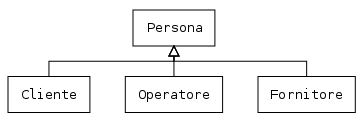
\includegraphics[width=10cm]{images/diagrams/persona.png}
		\end{center}
		
		Ad ogni \emph{Persona} saranno associati uno o più \emph{Recapiti}.
		
		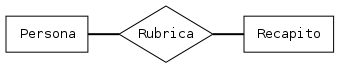
\includegraphics[width=11.5cm]{images/diagrams/persona_recapito.png}
		
		Possiamo concludere lo sviluppo della struttura del diagramma ER affrontando la questione delle transazioni. Avviene una \emph{Transazione} ogni volta che viene versato un acconto per un \emph{Preventivo}, ogni volta che viene saldata la \emph{Fattura} di una \emph{Prestazione}, ogni volta che viene pagato un \emph{Ordine} ed ogni volta che viene pagato il salario di un \emph{Operatore}.

		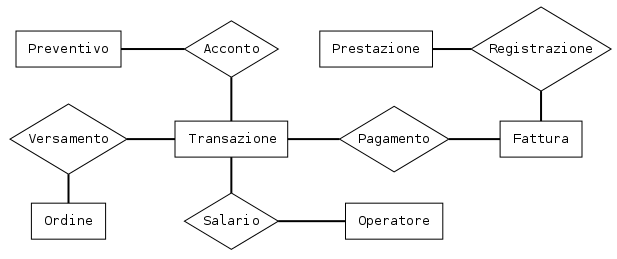
\includegraphics[width=11.5cm]{images/diagrams/transazione.png}
		
	\subsection{Scheletro dello Schema ER}
	
		Il diagramma in figura \ref{fig:scheletro_er} rappresenta lo scheletro dello schema ER.
		
		\begin{sidewaysfigure}
			\centering
			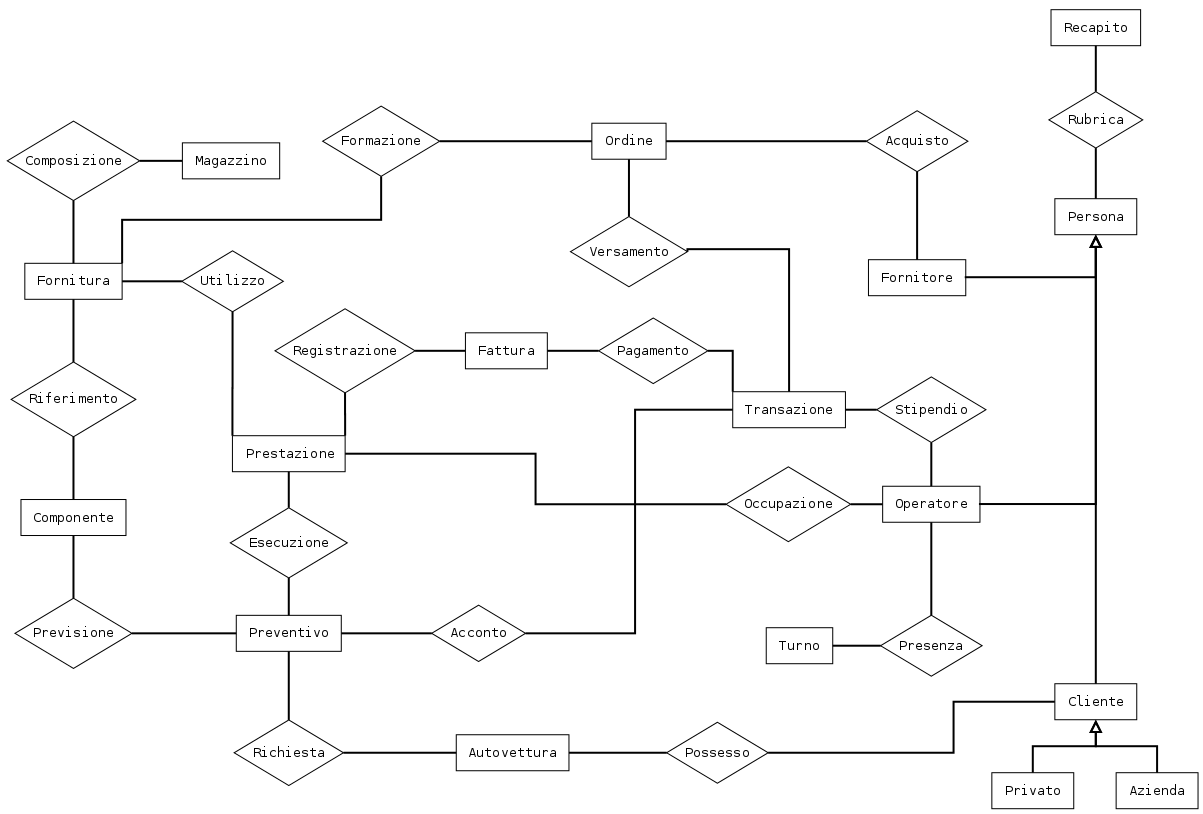
\includegraphics[width=20cm]{images/diagrams/schema.png}
			\caption{Scheletro del diagramma ER}
			\label{fig:scheletro_er}
		\end{sidewaysfigure}
	
	\subsection{Sviluppo delle Componenti dello Schema}
	
		Ottenuto lo scheletro generale del diagramma ER procediamo a raffinarne i componenti, aggiungendo attributi ed esplicitando le cardinalità delle relationship introdotte.
		
		\begin{description}
			\item[NB]
				Ogni generalizzazione effettuata è da considerarsi totale.
		\end{description}
		
		\subsubsection{Persona}
		
			In figura \ref{fig:persona} troviamo lo sviluppo degli attributi dell'entità \emph{Persona} e delle relative entità che la estendono.
						
			\begin{figure}[H]
				\centering
				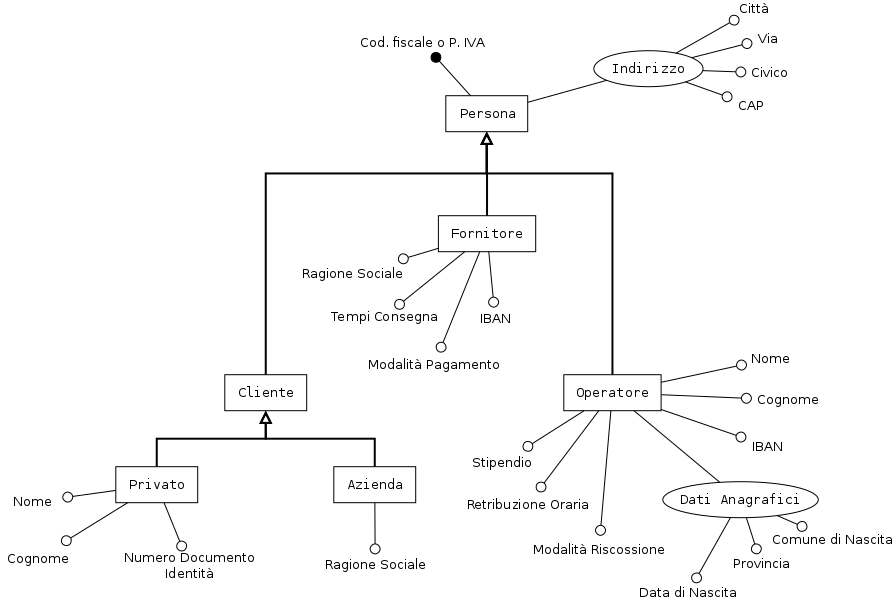
\includegraphics[width=12cm]{images/finitures/persona.png}
				\caption{Sviluppo di Persona}
				\label{fig:persona}
			\end{figure}
			
			Di ogni \emph{Persona} coinvolta nelle attività dell'azienda, suddivisibili in \emph{Clienti}, \emph{Fornitori} ed \emph{Operatori}, è necessario memorizzare all'interno della base di dati il codice fiscale e l'indirizzo di riferimento.		

	
	\subsection{Analisi Qualitativa dello Schema ER}
	
	\subsection{Dizionario dei Dati}
		
		\subsubsection{Entità}
		
			\begin{longtable}{| p{2.5cm} | p{4.5cm} | p{2cm} | p{2.5cm} |}
				\hline
				
					\textbf{Nome} & \textbf{Descrizione} & \textbf{Attributi} & \textbf{Identificatore} \\ \hline
					
					Nome entità & 
					Descrizione entità & 
					Attributi entità & 
					Identificatore entità
					\\
					
				\hline
			\end{longtable}
		
		\subsubsection{Relazioni}